%TEX root = ../dissertation.tex

\chapter{State of the Art}
\label{chapter:stateoftheart}
The first part of this review focus on the history of planning description
languages and their main features and drawbacks, as well as the recent
breakthroughs featuring stochastic planning languages.
The discussion followed next reflects upon the most recent results in
planning competitions\footnote{The main focus of the review will be about
International Planning Competitions from International Conference on Autonomous
Planning and Scheduling (ICAPS). More details at
\url{http://www.icaps-conference.org/index.php/Main/Competitions}},
not only the winners but also the other contestants and their attempted
methods/solvers to solve the problem in hands.

Finally, it will be discussed what has been done in the field of Symbiotic
Autonomy.

\section{Planning Representation Languages}
Since the 70's with STRIPS \cite{Fikes1971} there has been a major effort to
represent the \textit{physics} of the domains, giving expressiveness to which
predicates are available, what actions can be executed in some state and what
are their effects on their world model, and at the same time, avoiding the
frame problem.

With the rise of planning competitions in the 90's, the scientific community
wanted to give a sense of neutrality between the part of the program that does
the solving of the problem, that is, the one involved in choosing which actions
to perform to attain some goal, \textit{the solver}, and the one which describes
how the world changes in the agent's model, \textit{the planning representation
language}.

\subsection{Planning Domain Definition Language}
Planning Domain Definition Language (\textit{PDDL}) was designed by
Drew McDermott et al. \cite{McDermott1998} to standardize
the planning language used for the International Planning Competition in 1998,
providing a common ground for all the competitors, allowing for a clear
comparison between them and boost the sharing experience of
problems and algorithms between fellow researchers.

\textit{PDDL} separates the planning problem in two major groups,
the domain description file and the problem description file.

In the domain description file it is described:
\begin{itemize}
    \item The name of the physical domain.
    \item Set of requirements (here can appear any number of requirements by
    writing down a keyword starting with a colon following the
    \textbf{:requirements} keyword, also known as \textit{requirement flag}).
    \item Object types are enumerated (\textit{object} and \textit{number}
    object types are already included) by writing down after the \textbf{:types}
    keyword the available types in the domain.
    \item Definition of constants, symbols that have the same meaning in all
    problems in this domain.
    \item Available predicates of the domain are detailed combining their
    required parameters with the type of object they insert into.
    \item Possible actions applicable to the domain are described. It starts
    by choosing a name for the action after \textbf{:action} in addition to the
    parameters given as arguments.The preconditions for that action are defined
    next after \textbf{:precondition} followed by the keyword \textbf{:effects}
    and its effects.
\end{itemize}
It can be seen next a general scheme of the domain description file with the
most common keywords in Appendix \ref{code:pddl_code_general}.

As it has been said earlier, \textbf{PDDL} also includes a problem from a
specific domain, where it is outlined the objects present in this instance, the
initial state and the goal to be reached. The initial state description includes
a list of ground atoms that are true in the initial state, making all
the other atoms false (this can be overriden by writing \textbf{:open-world} in
the requirements of the domain). All predicate's arguments in the goal
description must be grounded. The template for a problem instance in
\textit{PDDL} is showed in Appendix \ref{code:pddl_problem}.

The solution to the problem is given by a sequence of actions such the series of
actions is possible given the initial situation and \textbf{:goal} is true in
the resulting set of actions that lead to that situation.

As it can be seen in the history of planning competitions, \textit{PDDL} had
great success in providing that needed common ground for researchers.
However, it did not stay frozen in time, it has been evolving from the needs of
expressiveness in planning domains, from one competition to another. Featured
next are the most important remarks about the updates on \textit{PDDL}:
\begin{itemize}
    \item In 2001, it was introduced \textit{PDDL2.1} \cite{Fox2003} which
    introduced durative actions with continuous effects, objective functions for
    measuring the quality of plans and numerical fluents. However, the concept
    of durative actions created some backlash from certain members of the
    scientific community, with Fahiem Bacchus \cite{Bacchus2003} claiming:
    '\textit{Planning domains, even simplified ones designed for research, can
    be modeled in many different ways, and I believe that it is better to
    produce more robust models with simpler languages than to develop languages
    with features that are not really needed.}'.
    \item For the planning competition in 2004, which concentrated on planning
    in temporal and metric domains, \textit{PDDL2.2} \cite{Edelkamp2004} was
    published. The core features were derived literals and timed initial
    literals. Derived literals are interesting on its own right by modeling
    the transitivity property of relations. The latter provides knowledge about
    facts that will be true or false at certain time points known in advance to
    the planner.
    \item In 2005, Gerevini and Long \cite{Gerevini2005} proposed an extension
    to the language by adding soft and strong constraints on plan trajectories,
    abling to express preferences over possible actions and intermediate states
    reached by the plan. The same was defined for goals. Strong constraints and
    goals must always be satisfied where soft constraints and goals serve the
    purpose of finding the most desirable plan. This is done by using weights
    on the plan metric expression, where the best plan is the one that optimizes
    that same expression. The language was defined as \textit{PDDL3.0} and was
    chosen as the one to represent planning domains and problems in the fifth
    International Planning Competition, 2006.
    \item The latest iteration of the planning language is \textit{PDDL3.1}
    \cite{Kovacs2011} and has been used in the deterministic track from the
    previous two International Planning Competitions in 2011 and 2014.
    However, information on temporal semantics of object fluents needs further
    work as well as the use of unknown values below needs\footnote{More info in
    \url{http://ipc.informatik.uni-freiburg.de/PddlExtension}}.


\end{itemize}
It is from that need of expressiveness in certain domains, the language
mentioned next is born.

\subsection{Probabilistic Planning Domain Definition Language}

In the fourth International Planning Competition, 2004, it was introduced for
the first time a probabilistic track where contestants would be able to solve
probabilistic and decision theoretic planning problems. To generalize
that sort of domains into a planning language, it was made an extension to
\textit{PDDL} which increased the ability to describe problems of that
particular kind of domains. From this need, \textit{PPDDL1.0} \cite{Younes2004}
was born as an extension of \textit{PDDL2.1}, capable of describing
\textit{MDP's}. Being an extension to \textit{PDDL2.1}, the previous syntax is
mantained with the addition of some important syntactic extensions, as the
following:
\begin{itemize}
    \item \textit{Probabilistic Effects: } This means that the effect of an
    action has a probabilistic outcome with the requirement of the following
    syntax in the effect keyword of an action:\\
    \centerline{\textit{(probabilistic $p_1$  $e_1$  ...  $p_k$  $e_k$)}}
    This means that effect $e_j$ has probability $p_j$ of occurring. What must
    be always guaranteed is that each event has a positive or zero probability
    of occurring and the sum of all events' probabilities must sum to 1. This is
    done by describing the set of probability-weighted outcomes for a
    probabilistic-effect pair. This change made possible to encode a large
    number state variables in a single action template.
    \item \textit{Rewards: }can be encoded as \textit{fluents} and are
    associated with state transitions. The language also restricts the use of
    the fluent \textit{reward} to describe the total accumulated reward
    (starting with 0 value) from the start of the planning problem until the
    current moment and is not usable in the preconditions and effects of
    actions.
    \item \textit{Probabilistic Initial Conditions of a Problem: }This means
    that the grounding of a problem is not necessary to solve it.
\end{itemize}

It is worthy of mention that this language was also used in the subsequent
International Planning Competition, in 2006, showing the success of this
planning language, built upon a well known and standardized framework by
researchers of the field.

\subsection{Relational Dynamic influence Diagram Language}
From journal article of Sanner \cite{Sanner2008} in 2008, many interesting
real world domains were very difficult or even impossible to model
with the current state of \textit{PPDDL}, some of them include:
\begin{itemize}
    \item \textit{Domains with multiple concurrent actions with uncertain
    outcomes:} with this kind of situation, we can have a number of joint
    actions exponential with number of concurrent actions. So, enumerating all
    the possible joint actions or outcomes would prove to be an impossible task
    for a lot of the previous state of the art planners, turning this into a
    very interesting challenge. So concurrency is a must in this probabilistic
    environment.
    \item \textit{Continuous action-state spaces:} following real world planning
    problems which are in most of the cases continuous action-state
    \textit{MDP}s. Making planners for this kind of problems is not a trivial
    task, so it is likely that the Bellman equations give better solutions.
    \item \textit{Lack of goals:} when the planner has the general task of
    maximizing the expected reward or by optimizing a complex expression.
    \item \textit{Multiple Agents}.
    \item \textit{High Dimensional POMDP}s.
    \item \textit{External Actions and Events}.
\end{itemize}
All these domains can not be described in \textit{PPDDL}. This has happened
because from \textit{PDDL2.1} until this point, \textit{PPDDL} became static
unlike its deterministic counterpart which suffered several modifications, year
after year. Coupling this reason with the ones already talked before, it seems
clear that starting from a clean sheet would be the most successful approach to
handle domains with such a complex nature.

Hence, in order to introduce domains with the kind of features into the Eighth
\textit{IPC} in 2011, Sanner described a new planning language, Relational
Dynamic Influence Diagram Language\footnote{Multiple examples, documentation and
source can be found in \url{https://github.com/ssanner/rddlsim}} (\textit{RDDL})
\cite{Sanner_RDDL}, expecting to promote research into solving lifted (without
grounding) \textit{MDP}s and \textit{POMDP}s by tackling them with a relational
description language, giving rise to scalable and compact domain reprentations.
It describes states, actions and observations as parameterized variables (are
used to describe the domain in a lifted manner) and the evolution of a process
as a function of the next state, knowing the current state and action variables.
With this type of description of the domain, it can be converted to a graphic
representation, using a Dynamic Bayes Net (\textit{DBN}). The objective function
stipulates how the rewards of the domain should be optimized in the planning
problem, to maximize the expected reward.

With \textit{RDDL}, everything is a parameterized variable, whether it refers to
action, state, observation and intermediate fluents or constant nonfluents.
These fluents can be binary, multi-valued, integer and continuous. The semantics
of the language could be interpreted as a ground \textit{DBN} with support for
factored variables. In the mathematical domain, there is support for the
classical logical expressions (conjunction, disjunction, negation, implication,
equivalence and logical quantifiers), arithmetic operators, flow control and
most common probability distributions.

It is also possible to have classical planning along with \textit{POMDP}s,
including goals and preferences, finite horizon and (un)discounted rewards.
Constraint description on states and actions is also available.

A simple, commented example can be seen in appendix \ref{code:rddl}.

\newpage

\section{Planning Solvers}

The planning solvers which will be featured next are related to the two previous
\textit{IPC}s (The Seventh \cite{Vallati2015}, and The Eighth \cite{Coles2012})
and another one that won every competition (officially and unofficially) until
then. Thus, the discussion is started by explaining that solver, called
\textit{FF-Replan}, and then multiple planners based on Monte Carlo Tree Search
algorithms are described. The ones chosen to be discussed here have won
planning competitions or have approached the planning problems in an unorthodox
manner and deserve an honorable mention.

\subsection{FF-Replan}
This algorithm \cite{Yoon2007} for solving planning problems starts by
transforming a probabilistic planning problem (with the domain description and a
problem instance) into a deterministic one. This is accomplished while using a
heuristic that only takes into account the outcome of an action with the biggest
probability of occurring (another heuristic exists, which considers each outcome
as a different action, using much more computational resources and not as
scalable to bigger planning problems). Then, an ordered plan is found by using a
deterministic planner, and during the execution of this plan, if something
happens that leads the agent to an unexpected current state, a new plan is made
using the current state as the initial one. This process is repeated until the
agent reaches its goal state. Hence, planning and execution is performed until a
goal is reached.

This solver was very successful while the planning language was \textit{PPDDL},
as the domains could not capture most of the events that can happen in
environments with uncertain action effects and observations. At the time, other
state of the art solvers were using planners that relied on the optimization of
value functions and policies for the entire state space whereas this planner
focused on getting heuristics which enabled a reduced exploration of the state
space into the goal.

\subsection{Monte-Carlo Tree Search}

Recent methods have successfully applied Monte-Carlo Tree Search methods in
order to find which action will lead to the highest expected outcome. They work
with a best-first search criteria and stochastic simulations and starts with the
node of the current state, then the algorithm runs on a cycle between
\textbf{selection} (selecting the node that will be considered next, taking into
account the exploration \& exploitation principle), \textbf{expansion} (if a new
state is found, add a new node, corresponding to that state, to the tree),
\textbf{simulation} (Using some kind of heuristic, make a simulation of a plan
using the tree) and finishing each step of the loop by \textbf{backpropagating}
the result of the simulation to all the nodes which were transversed.

\begin{figure}[H]
    \centering
        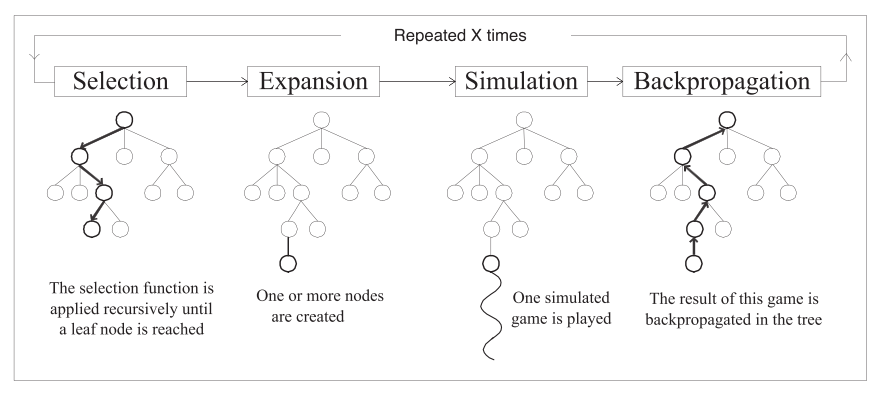
\includegraphics[width=14cm]{images/monte_carlo}
        \caption{Graphical procedure of Monte-Carlo Tree Search used on game
        playing. Image taken
        from \cite{Chaslot2008}. }
        \label{fig:monte_c}
\end{figure}

\textit{PROST}\footnote{Full source available at
\url{http://prost.informatik.uni-freiburg.de/}} is a planners that
uses Monte-Carlo Tree Search with a successor node choosen based on upper
confidence bounds applied to trees (\textit{UCT}) for solving \textit{MDP}s.
\textit{UCT} always returns a decision which is not random and finishes based on
a given timeout parameter.
Working with rollouts, in each one of them, the nodes of the tree are
transversed from the root until a terminal node. By distinguishing between
decision nodes (only has a successor for a given action) and chance nodes
(multiple successors for one action), the following procedure can be made:
\begin{itemize}
    \item on a decision node: always choose successors that gave high rewards or
    the ones which have been rarely visited, based on the previous rollouts.
    \item on a chance node: the prefered successor will be taken by sampling the
    transition probability.
\end{itemize}
Another important remark about the algorithm is that it gives more importance to
decisions closer to the initial state.\\


Another algorithm relevant for this discussion is Determinized Sparse Partially
Observable Tree \cite{Somani2013} \textit{DESPOT} which is appropriate to solve
\textit{POMDP}s, handling problems with high dimensionalities and
action-observation histories by using an online planning method. This means that
planning is interlaced with execution over and over until a terminal state is
reached, finding only the next action that should be made for the current
belief using only information about the beliefs near this one. Therefore, the
belief tree is built, starting from the current belief and lookahead is
performed to find a policy that maximizes the value function.


\newpage

\section{Symbiotic Autonomy}
In this section, it will be discussed the research already developed in the field
of Symbiotic Autonomy, which is highly correlated to the main problem to be
\textit{solved}. For the most part, the work being done by \textit{CORAL}
group (from Carnegie Mellon University), led by Professor Manuela Veloso, has
been pushing the research of this area forward.

In activities where there is a symbiotic relationship, all the agents in the
world model of the robot are usually performing their own asynchronous actions,
and each agent is influenced by the outcome of the other agents' actions.
However, all agents actively cooperate with each other, by communicating,
requesting and providing help.
As said earlier, agents with this type of relationship can ask or receive help
from each other on actions they could not have performed by themselves,
overcoming their limitations. Each agent can help the other one by: performing
an action for the first agent; increasing the first agent's capability to
perform an action.

By interacting in an environment with multiple human agents and possible
actions, it can exist a lot of possible plans usable by the mobile robot agent,
establishing this situation as a planning problem, where each agent has a cost
associated to his state. Hence, each agent will perform the set of actions that
minimize the cost of each others' state in order to achieve the goal.

Now, it seems useful to introduce the concept of \textit{capability}: the
probability of an agent to complete an action. If this probability is zero, it
is impossible that this agent can perform successfully the action to be taken.
Conversely, if the probability is bigger than zero but lower than one, there is
a chance that this action would not be completed by the agent. If the
probability is equal to one, the agent can always perform this action
successfully. Another interesting concept which should be discussed is the
\textit{expectation}: the cost of achieving some particular state. This is the
variable that should be minimized while the mobile robot is planning.

The prime example of Symbiotic Autonomy is the project CoBot \cite{Rosenthal2010},
an autonomous robot agent that autonomously navigates in a building,
escorting a visitor to its scheduled meetings and fulfilling other needs which
he may have (e.g. feeling an absolute urge to drink coffee). In this task, the
visitor is not familiar with the building layout and the robot is unable to do
activities which require physical manipulation of objects. Similarly, the
robot could also be unsure about its exact location. On the other hand, the
human agent can easily manipulate objects around him and locate its exact
position on a map, while the mobile robot can plan optimal paths to multiple
locations. This seems like a perfect situation to test symbiotic autonomy on
a real testbed, analyze the convenience provided, its reliability to prevent
delays on the visitor schedule while minimizing the help requests to other
humans to increase its autonomy.

The planning language used by the \textit{CORAL} group for this task was
\textit{PDDL} with probabilistic extensions, estabilishing here a path to
improve the design of this domain by using a state of the art planning language
like \textit{RDDL}, boosting the expressiveness of what can be described in this
problem.

As it is not possible for a robot to be able to complete all tasks that he is
supposed to finish, due to the complex nature of the real world, this seems like
an advantageous alternative to successfuly complete most of the tasks assigned
to the mobile robot agent. On the other hand, as discussed before, this approach
raises new problems related to probabilistic planning which need to be properly
handled to give the best results possible in the current task. Furthermore, the
cost of asking for help to a human agent must be accurately determined, and may
even be different to each individual human agent \cite{Rosenthal2011}, adding
another level of difficulty to this problem.
